\subsubsection*{Perceptron Learning - Artificial Neuron}
In our Artificial Neural Network a Perecptron is an Artificial Neuron.
It is called an Artifical Neuron because it is a bio-inspired neuron which models
a neuron in the human brain in terms of inputs and output.

In Perceptron learning, we can take two inputs which are put towards an
activation function with a bias attached as seen in \ref{fig:perceptron}.
These inputs are multiplied by the weights that connect the input to the
activation function and depending on the result, the activation function may
fire an output. These inputs are either 1 or -1.

\begin{figure}
     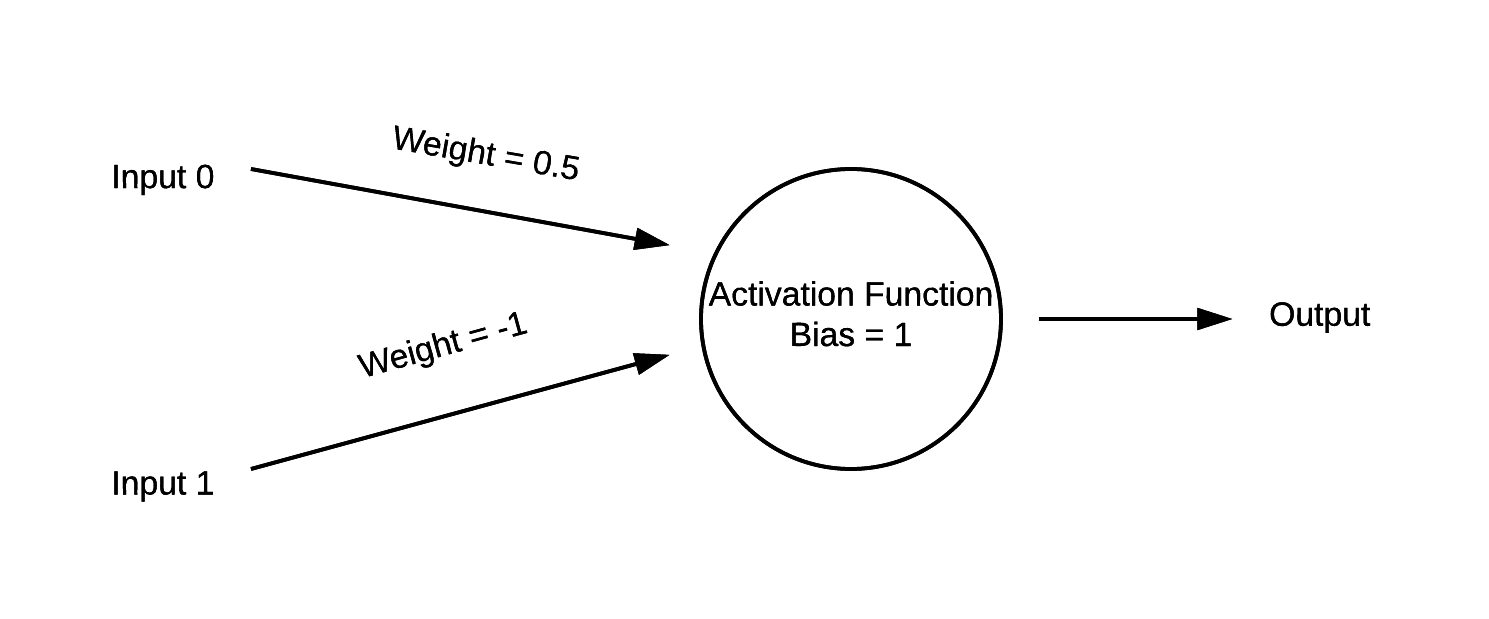
\includegraphics{Perceptron}
     \caption{Perceptron}
     \label{fig:perceptron}
\end{figure}

\begin{figure}
    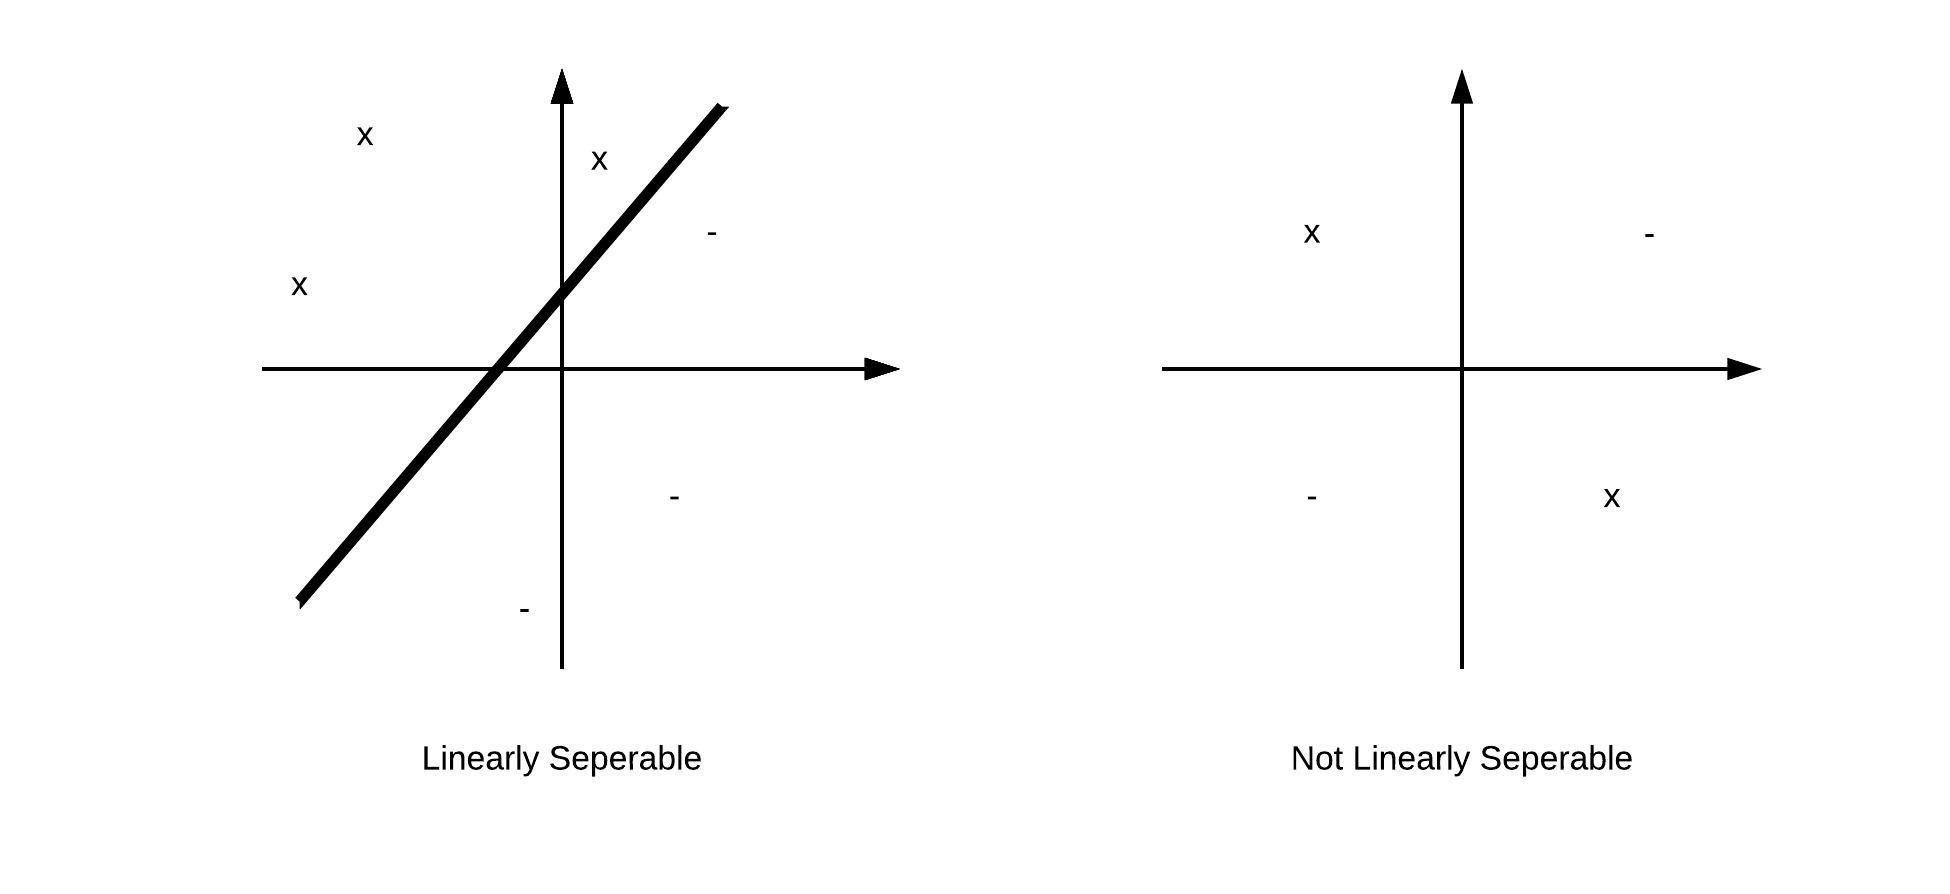
\includegraphics{LS}
     \caption{Linearly Separable, adapted from \textcite{MLANN}}
     \label{fig:ls}
\end{figure}

\begin{figure}
    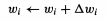
\includegraphics[scale=1.5]{ptr}
     \caption{The Perceptron Training Rule which changes weights, sourced from \textcite{MLANN}}
     \label{fig:ptr}
\end{figure}

\begin{figure}
    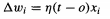
\includegraphics[scale=1.5]{ptr2}
     \caption{The Perceptron Training Rule condition, sourced from \textcite{MLANN}}
     \label{fig:ptr2}
\end{figure}

The Perceptron Training Rule is the means by which weights are selected to produce the correct output during training. As in \textcite{MLANN}, a common way to train a perceptron is t start with random weights and change them during training as per the training rule. This rule follows the formula in Figure \ref{fig:ptr} , where xi is the input and \ref{fig:ptr2} is valid. In \ref{fig:ptr2}, "t is the target output for the current training example, o is the output generated by the perceptron, and n is the positive constant called the learning rate" \textcite{MLANN}.
This Perceptron Training Rule assumes that there are two sets of instances, a
positive and negative set, and that they are linearly separable, as in Figure \ref{fig:ls}.

A perception is trained using supervised learning. When the perceptron
classifies a results, it is told if it is correct or not. If the result is
incorrect, weights are changed in value so that this error can be reduced
\textcite{AI}. 

The one major problem with perceptron learning and that is that it can't solve
the problem if there is not a clear linear separation between the classes. There
is a way in which we can attempt to solve this, through the delta rule. The
delta rule utilizes gradient descent to find the best weight for the training
samples \textcite{MLANN}. We will discuss gradient descent in the next section.

\subsubsection*{Multi Layered Perceptron}
Multi Layer Perceptrons (MLP) are made up of multiple layers of perceptrons connected
together and are used to combat non-linearly separable classes.
Firstly, we have an input layer, followed by one of more hidden layers and then
finally an output layer.
Any Neural Network with more than three hidden layers is categorised as a deep
layer.

The input layer of your network consists of the data you feed into the network
in order to classify it. The input layer passes this data to a hidden layer
whose purpose is to transform this data into something that the output layer can
understand. The output layer normally consists of a class prediction.

Multi Layer Perceptrons are a class of feed forward Artificial Neural Networks.
These means that the output of each perceptron feeds into an input in the next
layer of the network.

There is one large problem with MLP's and this is why Convolutional Neural
Networks (CNN) were created. If you attempting to classify images with an MLP then
each pixel in that image would have to be a separate input. This creates a
massive amount of neurons through all the layers and this isn't feasible. CNN's
solve this problem which we will discuss later.

\begin{figure}
    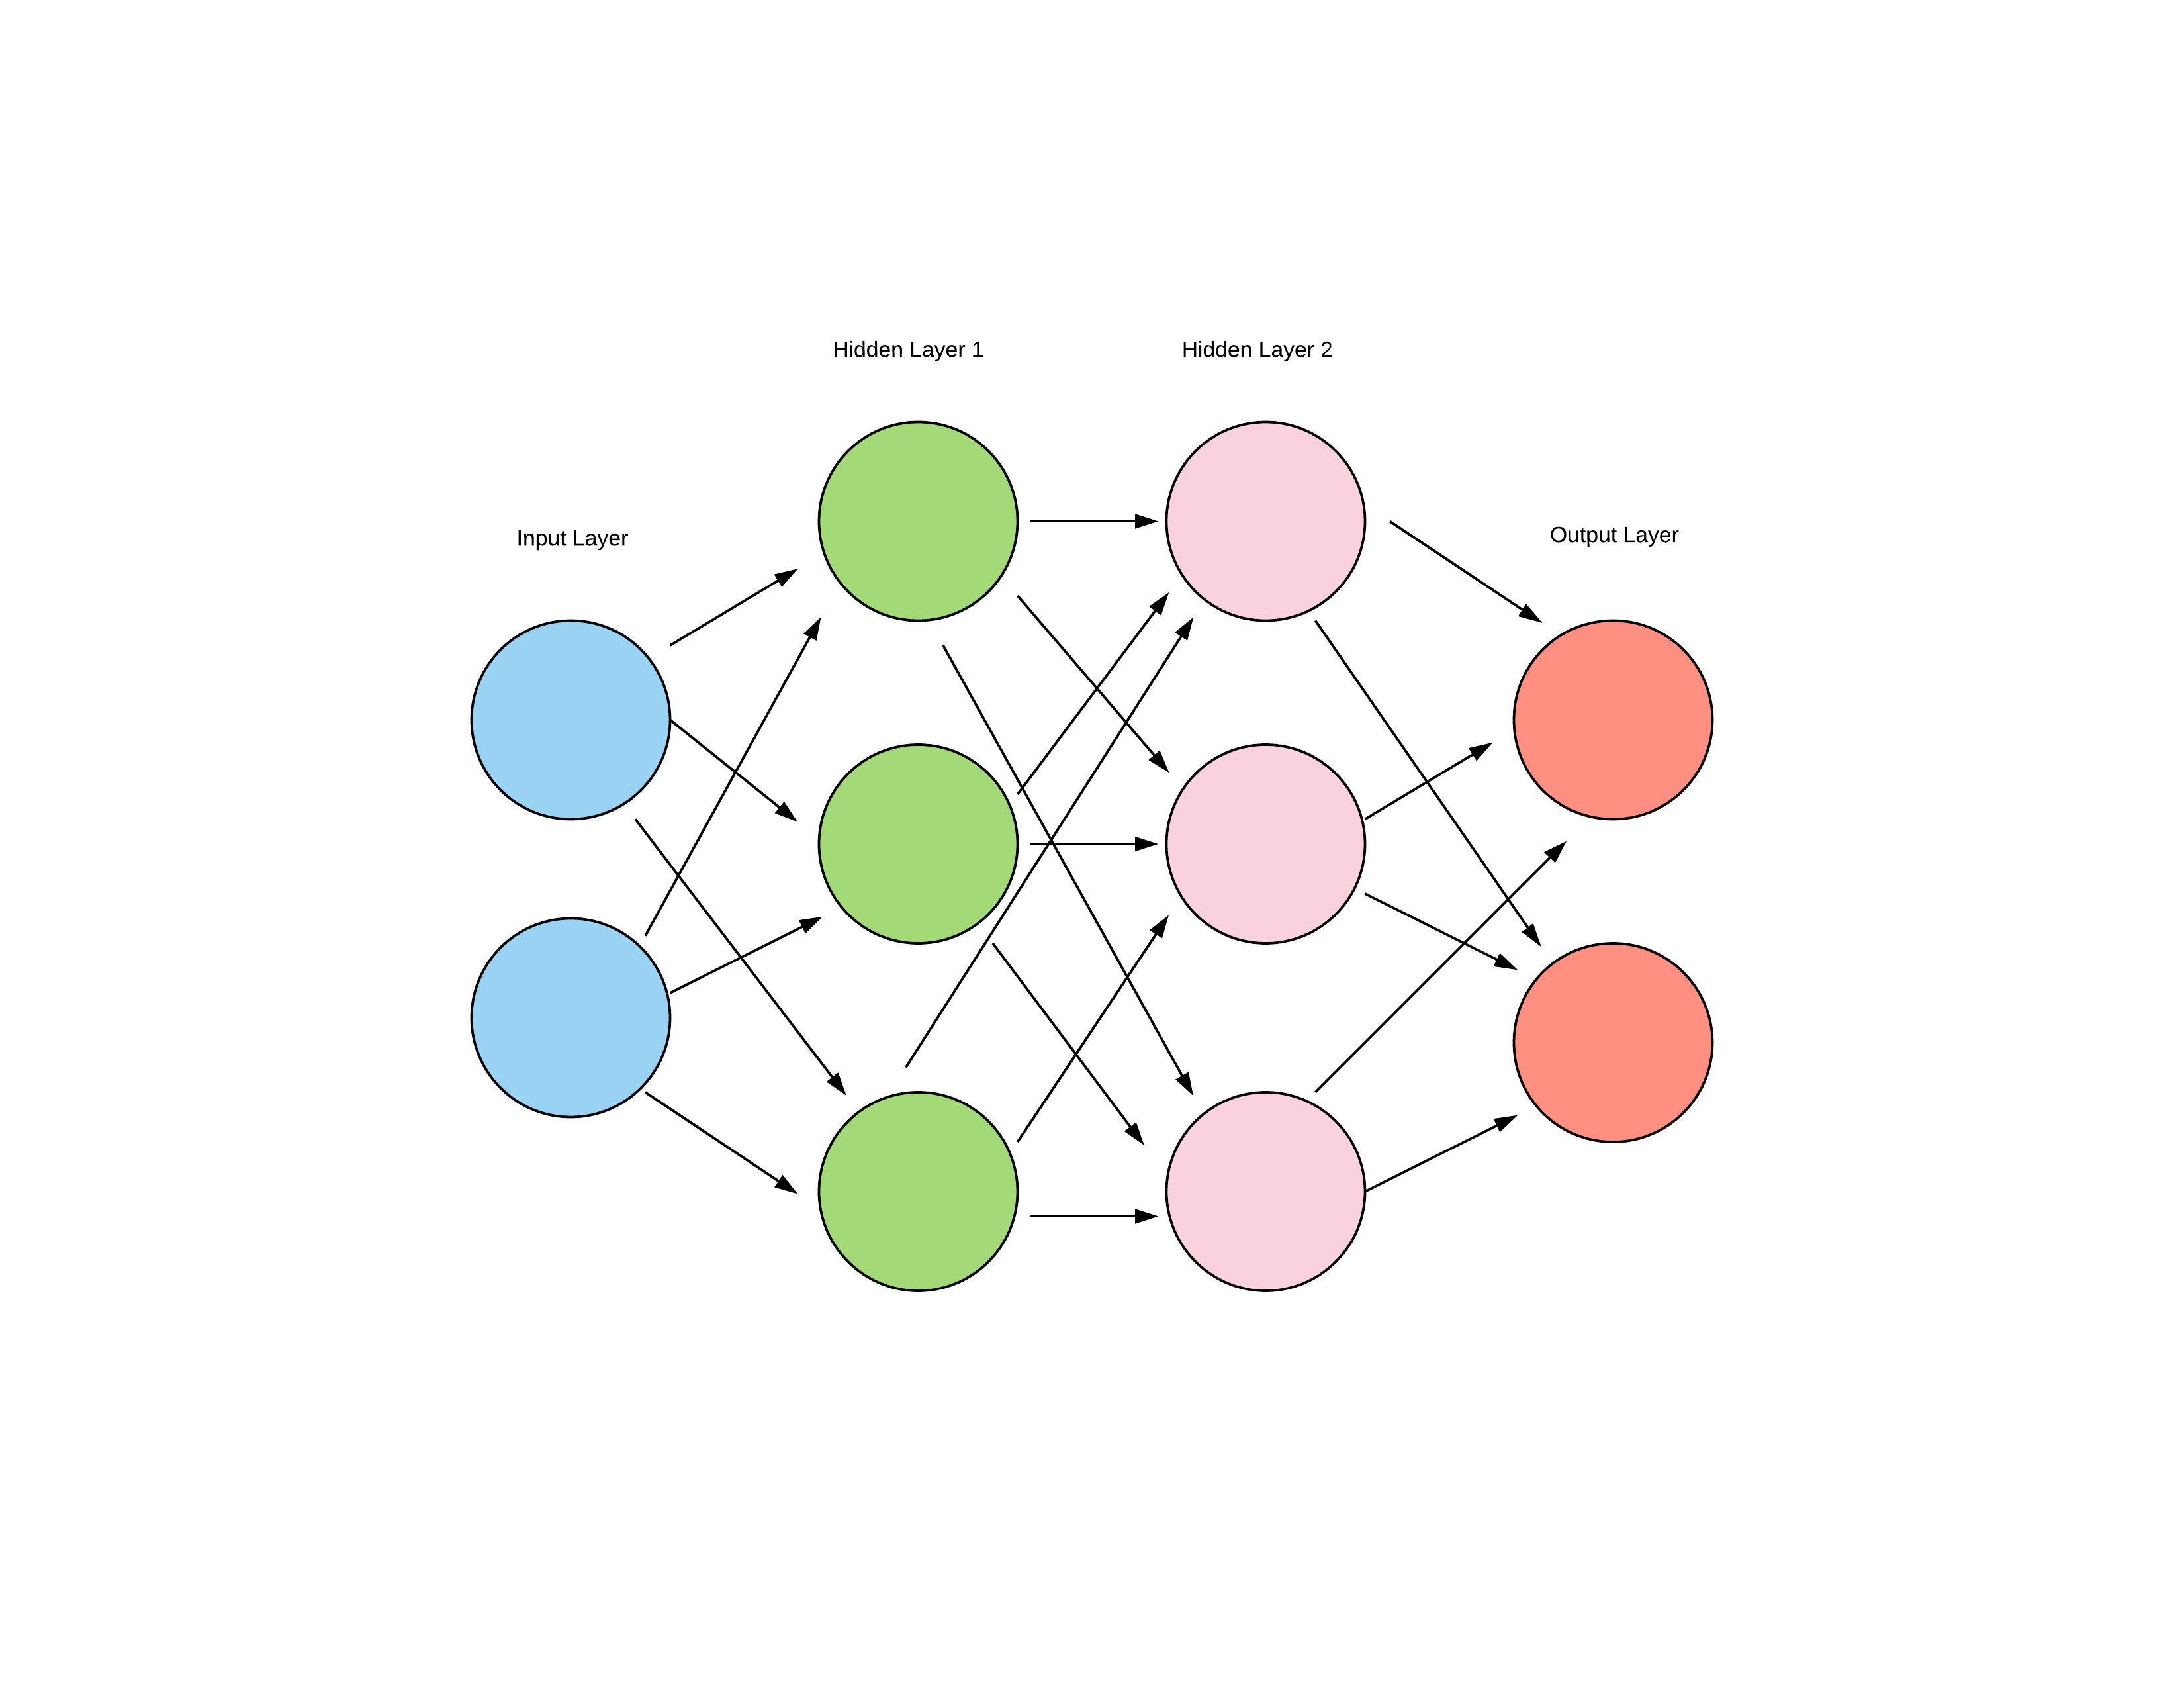
\includegraphics[width=150mm,scale=0.5]{mlp}
     \caption{Multi Layer Perceptron}
     \label{fig:mlp}
\end{figure}

